\documentclass[a4paper,14pt]{extreport}
	\usepackage[left=1.5cm,right=1.5cm,
	    top=1.5cm,bottom=2cm,bindingoffset=0cm]{geometry}
	\usepackage{scrextend}
	\usepackage[T1,T2A]{fontenc}
	\usepackage[utf8]{inputenc}
	\linespread{1.5}
	\usepackage[english,russian,ukrainian]{babel}
	\usepackage{tabularx}
	\usepackage{amssymb}
	\usepackage{color}
	\usepackage{amsmath}
	\usepackage{mathrsfs}
	\usepackage{listings}
	\usepackage{graphicx}
	\graphicspath{ {./images/} }
	\usepackage{lipsum}
	\usepackage{xcolor}
	\usepackage{hyperref}
	\usepackage{tcolorbox}
	\usepackage{tikz}
	\usepackage[framemethod=TikZ]{mdframed}
	\usepackage{wrapfig,boxedminipage,lipsum}
	\mdfdefinestyle{MyFrame}{%
	linecolor=blue,outerlinewidth=2pt,roundcorner=20pt,innertopmargin=\baselineskip,innerbottommargin=\baselineskip,innerrightmargin=20pt,innerleftmargin=20pt,backgroundcolor=gray!50!white}
	 \usepackage{csvsimple}
	 \usepackage{supertabular}
	\usepackage{pdflscape}
	\usepackage{fancyvrb}
	%\usepackage{comment}
	\usepackage{array,tabularx}
	\usepackage{colortbl}

	\usepackage{varwidth}
	\tcbuselibrary{skins}
	\usepackage{fancybox}
	\usepackage{spreadtab}
	\usepackage{xstring}
	\usepackage{fp}
	\usepackage{ulem}


	\usepackage{tikz}
	\usepackage[framemethod=TikZ]{mdframed}
	\usepackage{xcolor}
	\usetikzlibrary{calc}
	\makeatletter
	\newlength{\mylength}
	\xdef\CircleFactor{1.1}
	\setlength\mylength{\dimexpr\f@size pt}
	\newsavebox{\mybox}
	\newcommand*\circled[2][draw=blue]{\savebox\mybox{\vbox{\vphantom{WL1/}#1}}\setlength\mylength{\dimexpr\CircleFactor\dimexpr\ht\mybox+\dp\mybox\relax\relax}\tikzset{mystyle/.style={circle,#1,minimum height={\mylength}}}
	\tikz[baseline=(char.base)]
	\node[mystyle] (char) {#2};}
	\makeatother

	\definecolor{ggreen}{rgb}{0.4,1,0}
	\definecolor{rred}{rgb}{1,0.1,0.1}
	\definecolor{amber}{rgb}{1.0, 0.75, 0.0}
	\definecolor{babyblue}{rgb}{0.54, 0.81, 0.94}
	\definecolor{amethyst}{rgb}{0.6, 0.4, 0.8}
	\usepackage{graphicx}
	\usepackage{float}
	\usepackage{wrapfig}
	\usepackage{framed}
	%for nice Code{
	\lstdefinestyle{customc}{
	  belowcaptionskip=1\baselineskip,
	  breaklines=true,
	  frame=L,
	  xleftmargin=\parindent,
	  language=C,
	  showstringspaces=false,
	  basicstyle=\small\ttfamily,
	  keywordstyle=\bfseries\color{green!40!black},
	  commentstyle=\itshape\color{purple!40!black},
	  identifierstyle=\color{blue},
	  stringstyle=\color{orange},
	}
	\lstset{escapechar=@,style=customc}
%}


\begin{document}
\renewcommand{\bibname}{Список використаної літератури}

\pagecolor{white}

%----------------------------------------1
\newtcbox{\xmybox}[1][red]{on line, arc=7pt,colback=#1!10!white,colframe=#1!50!black, before upper={\rule[-3pt]{0pt}{10pt}},boxrule=1pt, boxsep=0pt,left=6pt,right=6pt,top=2pt,bottom=2pt}

\begin{titlepage}
	\begin{center}
	\large
	Національний технічний університет України \\ "Київський політехнічний інститут імені Ігоря Сікорського"


	Факультет Електроніки

	Кафедра мікроелектроніки
	\vfill

	\textsc{ЗВІТ}\\

	{\Large Про виконання курсової роботи \\
	з дисципліни: «Твердотільна електроніка-3»\\[1cm]

	Варіант №50


	}
	\bigskip
	\end{center}
	\vfill

	\newlength{\ML}
	\settowidth{\ML}{«\underline{\hspace{0.4cm}}» \underline{\hspace{2cm}}}
	\hfill
	\begin{minipage}{1\textwidth}
	Виконавець:\\
	Студент 3-го курсу \hspace{4cm} $\underset{\text{(підпис)}}{\underline{\hspace{0.2\textwidth}}}$  \hspace{1cm}А.\,С.~Мнацаканов\\
	\vspace{1cm}

	Перевірив: \hspace{6.1cm} $\underset{\text{(підпис)}}{\underline{\hspace{0.2\textwidth}}}$  \hspace{1cm}Л.\,М.~Королевич\\

	\end{minipage}

	\vfill

	\begin{center}
	2021
	\end{center}
\end{titlepage}

\newpage
\setcounter{page}{1}
%--------------------------------------------------------------------------------------2----------------------------------------------------------------------
\tableofcontents
%--------------------------------------------------------------------------------------3----------------------------------------------------------------------

\newpage
\setcounter{page}{1}

\newpage
\chapter{ВСТУП}

\newpage
\chapter{ТЕХНІЧНЕ ЗАВДАННЯ НА ПРОЕКТУВАННЯ}

\newpage
\chapter{АНАЛІЗ СХЕМИ}
%//////////////////
%////   1     ////
%////////////////
	\begin{figure}[h!]
	\center{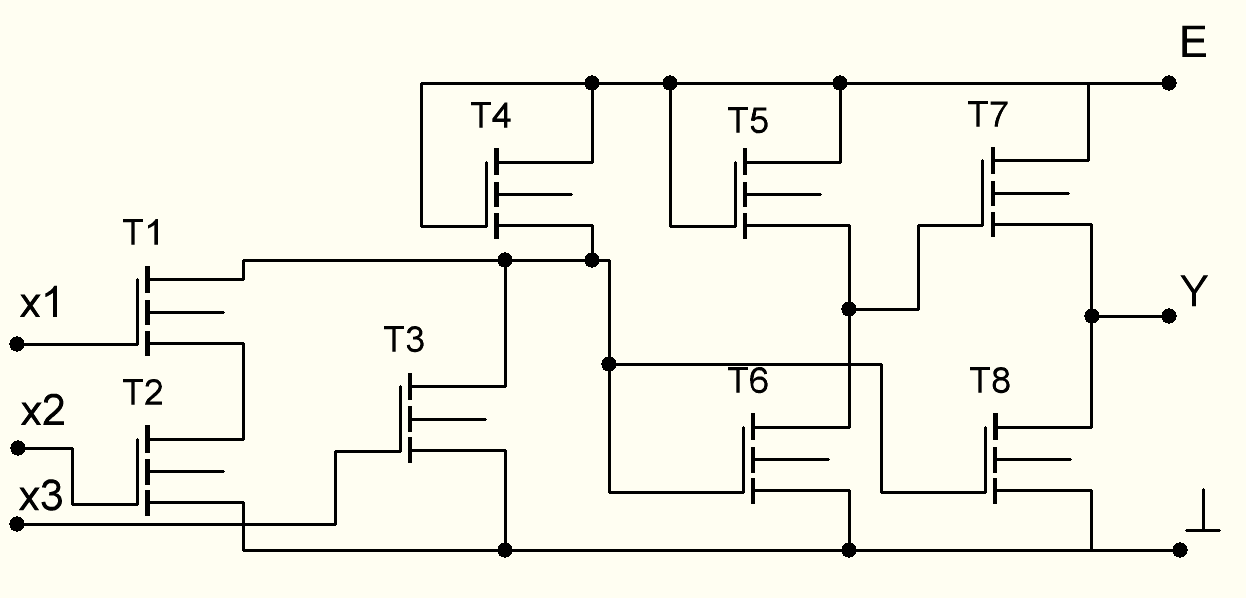
\includegraphics[width=1\linewidth]{1-a.png}}
	\caption{Прототип схеми.}
	\label{ris1}
	\end{figure}
	У мене за варіантом тип підкладки КЕФ, тобто n-тип підкладки, тоді $Rightarrow$ p-канал у транзисторах.

	\begin{figure}[h!]
	\center{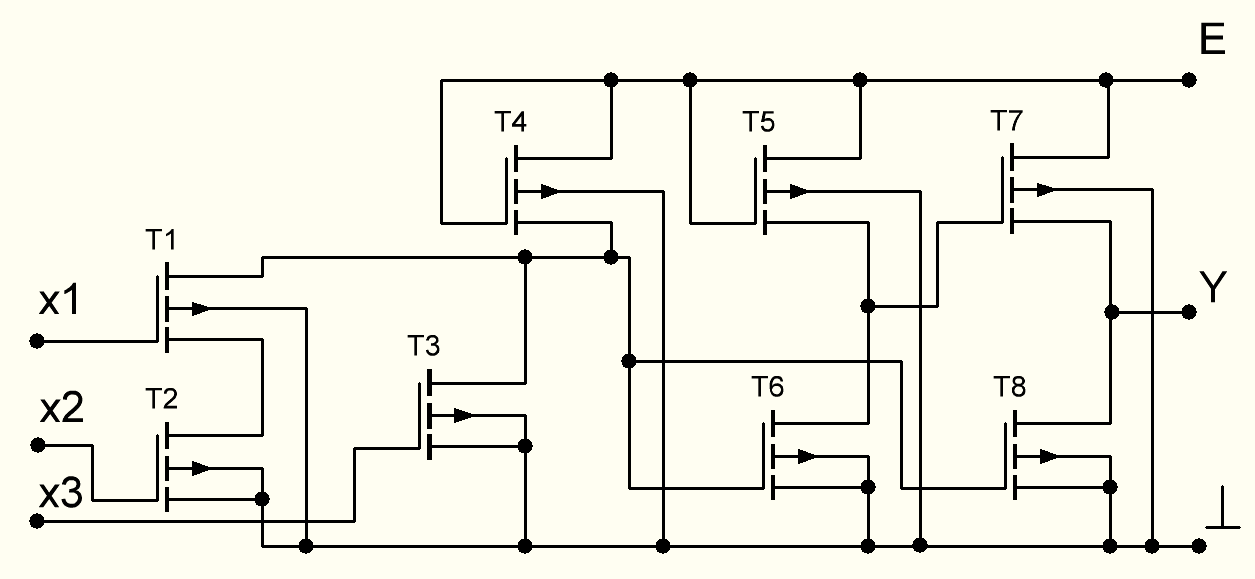
\includegraphics[width=1\linewidth]{2-a.png}}
	\caption{Електрична схема на основі прототипу.}
	\label{ris2}
	\end{figure}
	Оскільки у нас інтегральна мікросхема, то треба аби всі підкладки були підключені до спільного вивод, що і показано на рис.\ref{ris2}.\\

	Тепер переходимо до наступного завдання. Треба скласти таблицю істинності, але легше зробити це розбивши схему на каскади. Розглядати будемо спрощену модель схеми (бо так простіше), замінивши усі транзистори змінними резисторами, окрім T4 і T5. Так як у них затвор під’єднаний до стоку, то ці транзистори будуть грати роль нагрузки, тобто заміняємо їх звичайними резисторами.
	\newpage


	\begin{figure}[h!]
	\begin{center}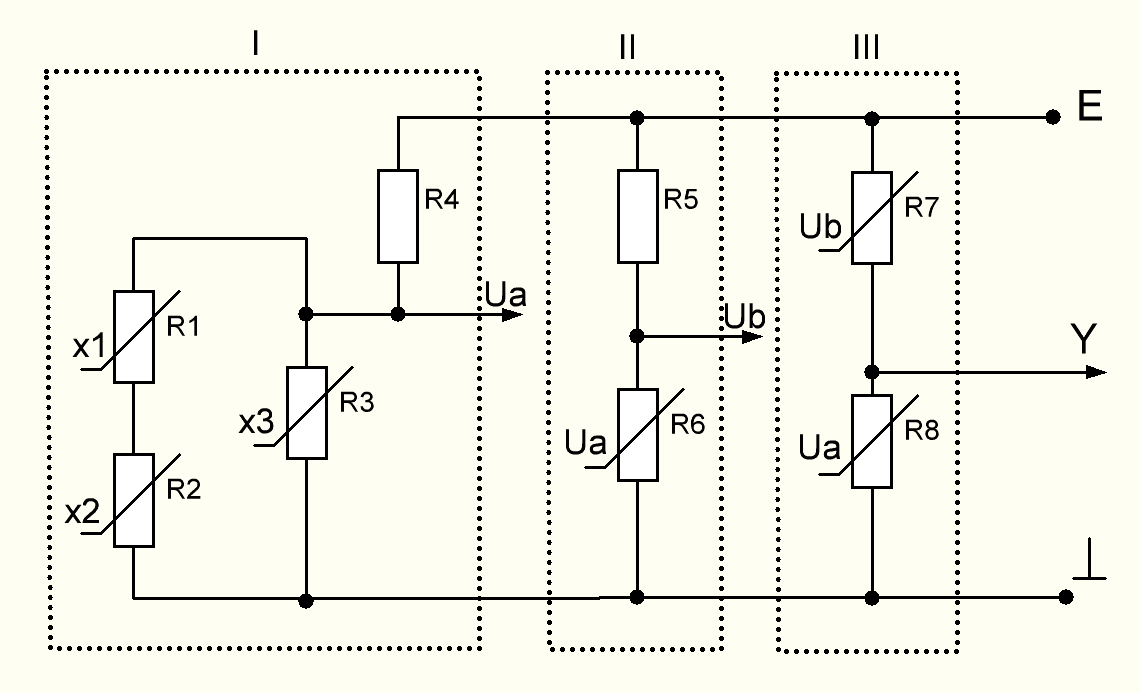
\includegraphics[width=1\linewidth]{3-a.png}\end{center}
	\caption{Спрощена модель.}
	\label{ris3}
	\end{figure}


	Бачимо, що у цій схемі всього три каскади. Розпочнемо з першого. У нас три змінних резистори, які можна об’єднати в один (спочатку R1 I R2, так як вони послідовно з'єднані, і потім з R3, так як паралельно підключені). Покроково це виглядатиме так:


	\newpage

	\begin{figure}[h!]
	\center{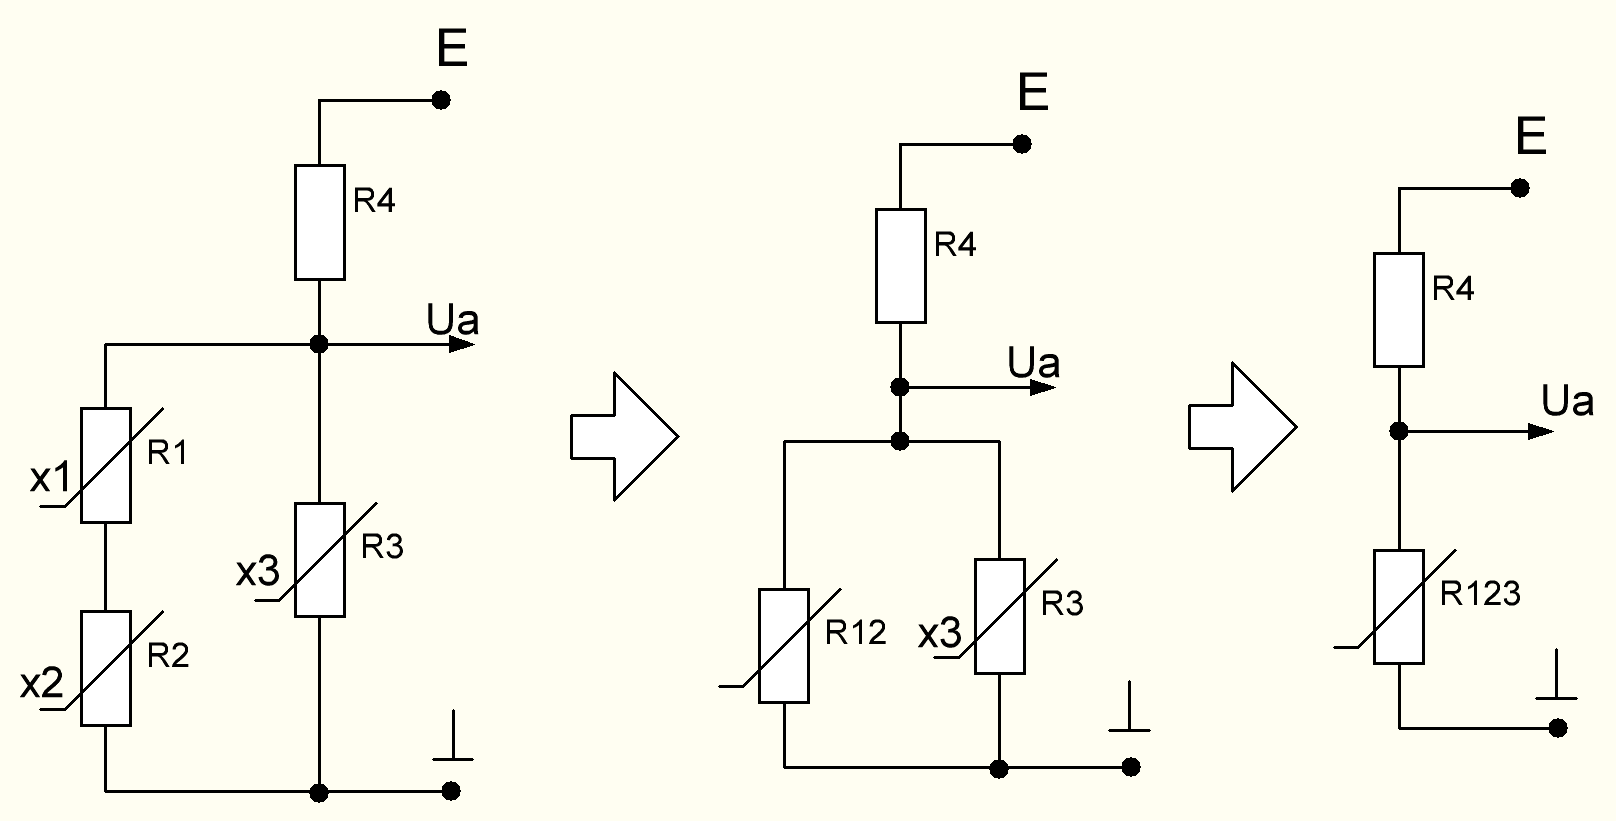
\includegraphics[width=1\linewidth]{4-a.png}}
	\label{ris4}
	\end{figure}

	\begin{align}
	  R_{12} = R_1 + R_2
	\end{align}
	\begin{align}
	  R_{123} = \dfrac{R_{12} \cdot R_3}{R_{12} + R_3} = \dfrac{R_{1}+R_{2} \cdot R_3}{R_{1}+R_{2} + R_3}
	\end{align}

	По нашому скороченню, у нас вийшов резистивний дільник напруги (по резисторам $R_{4}$ i $R_{123}$). Знаходимо напругу $U_a$.

	\begin{align}
	  U_a = \dfrac{R_{123} \cdot E}{R_{4} + R_{123}}
	\end{align}
	По цих формулах уже можемо складати таблицю істинності для першого каскаду. Аби було легше рахувати, приймемо, що $R_{3} \rightarrow 0$ , а потім, що $R_{3} \rightarrow \infty$.

	\begin{table}[h]
	  \begin{center}
	    \begin{tabular}{|c|c|c|c|c|}
	    \hline
	    $R_1 $  & 1 & 1 & 0 & 0 \\ \hline
	    $R_2 $  & 1 & 0 & 1 & 0 \\ \hline
	    $R_3 $  & 0 & 0 & 0 & 0 \\ \hline
	    $R_{123} $& 0 & 0 & 0 & 0 \\ \hline
	    $U_a  $ & 0 & 0 & 0 & 0 \\ \hline
	    \end{tabular}
	  \end{center}
	\end{table}
	Тепер для $R_{3} \rightarrow \infty$

	\begin{align}
	R_{123}=\dfrac{\left(R_{1}+R_{2}\right) \cdot R_{3}}{R_{3} \dfrac{\left(R_{1}+R_{2}\right)}{R_{3}}+R_{3}}=\dfrac{\left(R_{1}+R_{2}\right) \cdot R_{3}}{R_{3}\left(\dfrac{\left(R_{1}+R_{2}\right)}{R_{3}}+1\right)}=
	 \dfrac{\left(R_{1}+R_{2}\right)}{\left(\dfrac{\left(R_{1}+R_{2}\right)}{R_{3}}+1\right)}=\dfrac{\left(R_{1}+R_{2}\right)}{(0+1)}=R_{1}+R_{2}
	\end{align}



	\begin{table}[h]
	  \begin{center}
	    \begin{tabular}{|c|c|c|c|c|}
	    \hline
	    R1   & 1 & 1 & 0 & 0 \\ \hline
	    R2   & 1 & 0 & 1 & 0 \\ \hline
	    R3   & 1 & 1 & 1 & 1 \\ \hline
	    R123 & 1 & 1 & 1 & 0 \\ \hline
	    Ua   & 1 & 1 & 1 & 0 \\ \hline
	    \end{tabular}
	  \end{center}
	\end{table}



	Тоді, загальна таблиця разом з x1, x2, x3 матиме вигляд:


	\begin{table}[h]
	  \begin{center}
	    \begin{tabular}{|c|c|c|c|c|c|c|c|c|}
	    \hline
	    X1   & 0 & 0 & 0 & 0 & 1 & 1 & 1 & 1 \\ \hline
	    X2   & 0 & 1 & 0 & 1 & 0 & 1 & 0 & 1 \\ \hline
	    X3   & 0 & 0 & 1 & 1 & 0 & 0 & 1 & 1 \\ \hline
	    R1   & 1 & 1 & 1 & 1 & 0 & 0 & 0 & 0 \\ \hline
	    R2   & 1 & 0 & 1 & 0 & 1 & 0 & 1 & 0 \\ \hline
	    R3   & 1 & 1 & 0 & 0 & 1 & 1 & 0 & 0 \\ \hline
	    R123 & 1 & 1 & 0 & 0 & 1 & 0 & 0 & 0 \\ \hline
	    Ua   & 1 & 1 & 0 & 0 & 1 & 0 & 0 & 0 \\ \hline
	    \end{tabular}
	  \end{center}
	\end{table}


	Усе, таблиця істинності 1 каскаду зроблена. Далі переходимо до 2 і 3 каскаду:




	\begin{figure}[h!]
	\center{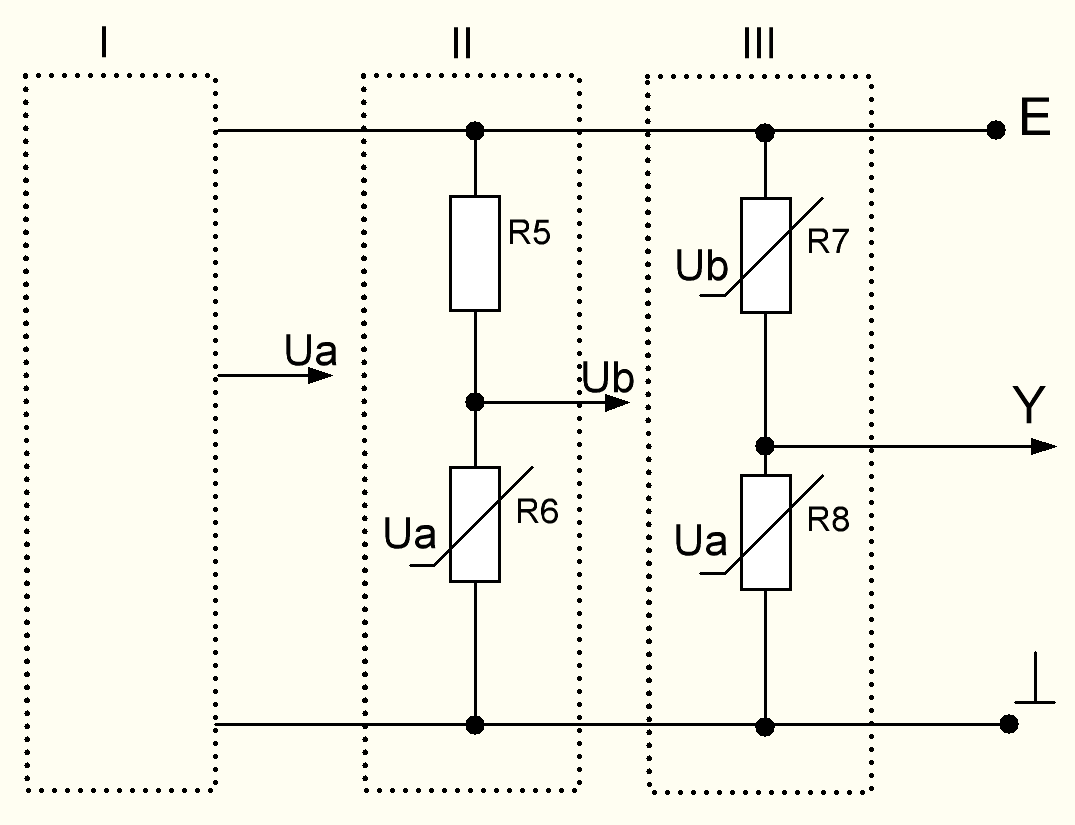
\includegraphics[width=0.7\linewidth]{5-a.png}}
	\label{ris5}
	\end{figure}
	Тут два дільники напруги. Можемо одразу скласти формули напруги для Ub та Y:
	\begin{equation}
	U_{b}=\dfrac{R_{6}}{R_{5}+R_{6}} \cdot E \quad Y=\dfrac{R_{8}}{R_{7}+R_{8}} \cdot E
	\end{equation}

	Складаємо таблицю істинності одразу для двох каскадів:

	\begin{table}[h]
	  \begin{center}
	  \begin{tabular}{|c|c|c|}
	  \hline
	  Ua & 1 & 0 \\ \hline
	  R6 & 0 & 1 \\ \hline
	  Ub & 0 & 1 \\ \hline
	  R7 & 1 & 0 \\ \hline
	  R8 & 0 & 1 \\ \hline
	  Y  & 0 & 1 \\ \hline
	  \end{tabular}
	  \end{center}
	\end{table}

	Таблиця істинності 2 і 3 каскаду є. Тепер об’єднаємо таблиці істинності першого і другого – третього каскадів:


	\begin{table}[h]
	  \begin{center}
	\begin{tabular}{|c|c|c|c|c|c|c|c|c|}
	\hline
	X1 & 0 & 0 & 0 & 0 & 1 & 1 & 1 & 1 \\ \hline
	X2 & 0 & 1 & 0 & 1 & 0 & 1 & 0 & 1 \\ \hline
	X3 & 0 & 0 & 1 & 1 & 0 & 0 & 1 & 1 \\ \hline
	Ua & 1 & 1 & 0 & 0 & 1 & 0 & 0 & 0 \\ \hline
	Ub & 0 & 0 & 1 & 1 & 0 & 1 & 1 & 1 \\ \hline
	Y  & 0 & 0 & 1 & 1 & 0 & 1 & 1 & 1 \\ \hline
	\end{tabular}
	  \end{center}
	\end{table}

	Ми побачили, що другий каскад інвертуючий, через що Ub має протилежні знаки відносно Ua, а третій каскад не є інвертуючим, тому і має те саме, що Ub.
	Далі складаємо логічну функцію по отриманій таблиці:
	\begin{equation}
	\begin{array}{l}
	Y=\bar{x}_{1} \cdot \bar{x}_{2} \cdot x_{3}+\bar{x}_{1} \cdot x_{2} \cdot x_{3}+x_{1} \cdot x_{2} \cdot \bar{x}_{3}+x_{1} \cdot \bar{x}_{2} \cdot x_{3}+x_{1} \cdot x_{2} \cdot x_{3}= \\
	=\bar{x}_{1} \cdot x_{3}++x_{1} \cdot x_{2} \cdot \bar{x}_{3}+x_{1} \cdot x_{3}=x_{3}+x_{1} \cdot x_{2} \cdot \bar{x}_{3}=x_{3}+x_{1} \cdot x_{2}
	\end{array}
	\end{equation}



	І далі, останній крок, малюємо логічну схему по формулі:


	\begin{figure}[h!]
	\center{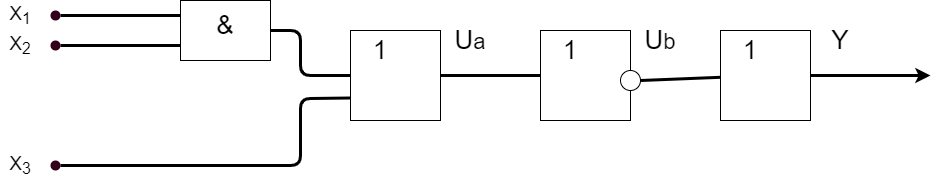
\includegraphics[width=0.9\linewidth]{courseW-a.png}}
	\label{ris6}
	\end{figure}


\newpage
\chapter{РОЗРАХУНОК ПОРОГОВОЇ НАПРУГИ ІНТЕГРАЛЬНИХ КОМПОНЕНТІВ СХЕМИ}
%//////////////////
%////   2     ////
%////////////////
	\begin{figure}[h!]
	\center{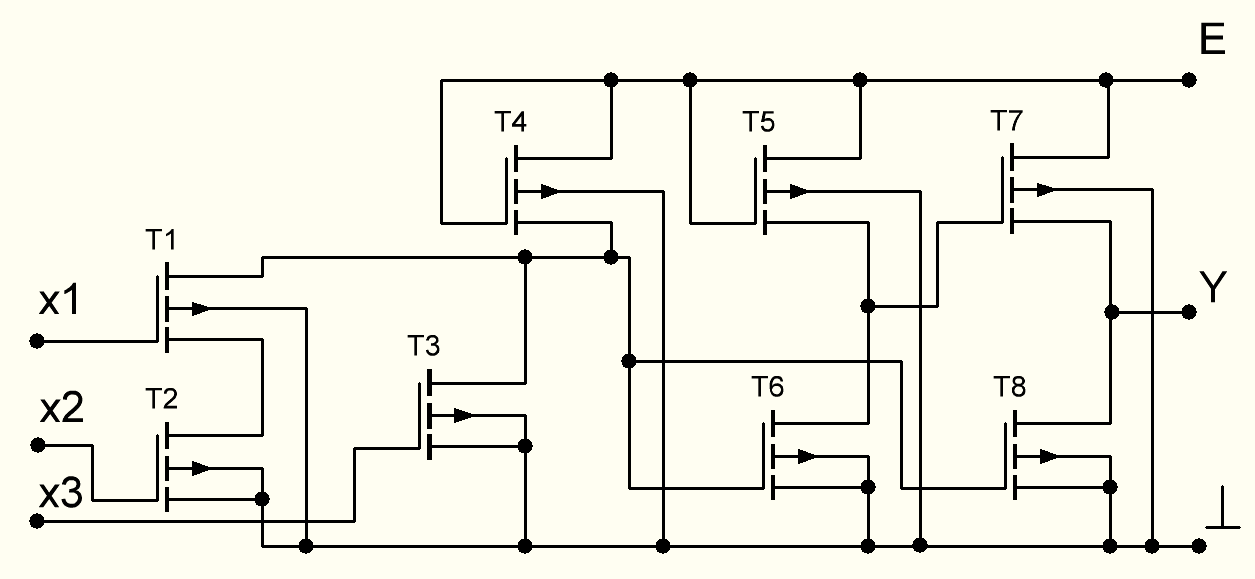
\includegraphics[width=1\linewidth]{1-b.png}}
	\caption{Прототип схеми.}
	\label{ris1}
	\end{figure}

	Треба записати формулу для пошуку порогової напруги. За варіантом  у мене КЕФ, тому формула буде наступною:
	\begin{equation}
	U_{n o p}^{0}=\phi_{M S}-\dfrac{q \cdot N_{S S}}{C_{o x}}-2 \cdot \phi_{F}-\dfrac{\sqrt{2 \cdot q \cdot \varepsilon_{0} \cdot \varepsilon_{S} \cdot N_{B}}}{C_{o x}} \cdot \sqrt{\left|2 \cdot \phi_{F}+U_{n}\right|}
	\end{equation}

	У цій формулі
	дано майже все, а точніше: $\quad N_{S S}=7,3 \cdot 10^{11} \text{см}^{-3}$
	$\varepsilon_{0}=8,85 \cdot 10^{-14} \Phi / \text{см}$
	$q=1,6 \cdot 10^{-19}\text{Кл}$
	$k_{B}=1,38 \cdot 10^{-23}$ Дж/К $, T=300 \mathrm{~K}, n_{i}=1,45 \cdot 10^{10} \mathrm{~cm}^{-3}, \varepsilon_{S}=11.8$
	Питома ємність шукається як
	\begin{equation}
	C_{o x}=\varepsilon_{0} \cdot \varepsilon_{o x} / d_{o x}=\dfrac{8,85 \cdot 10^{-14} \cdot 3,9}{10^{-5}}=3,45 \cdot 10^{-8}\text{ } \dfrac{\Phi}{\text{см}^{2}}
	\end{equation}

	Рівень Фермі у об'ємі кремнію:
	\begin{equation}
	\phi_{F}=\left(\dfrac{k_{B} \cdot T}{q}\right) \cdot \ln \left(\dfrac{N_{B}}{n_{i}}\right)
	\end{equation}
	I невідома сама концентрація $N_{B},$ тому користуємось наступною ф-ю:



	\vspace{0.5 cm}
	$\sigma=\dfrac{1}{\rho}=\left.q \cdot n \cdot \mu_{n}\right|_{n=N_{B}} \Rightarrow n=\dfrac{1}{\rho \cdot q \cdot \mu_{n}}=\dfrac{1}{5 \cdot 1,6 \cdot 10^{-19} \cdot 1500} \approx 8,3 \cdot 10^{14} \text{ }$ см $^{-3}$
	\vspace{0.5 cm}

	у формулі бело взято, що $\rho=5$ Ом$\cdot$см$, N_{B}=8,3 \cdot 10^{14}$ \text{ } см$^{-3}$\\

	Тобто, рівень Фермі тоді буде:\

	$$\phi_{F}=\left(\dfrac{k_{B} \cdot T}{q}\right) \cdot \ln \left(\dfrac{N_{B}}{n_{i}}\right)=\dfrac{1,38 \cdot 10^{-23} \cdot 300}{1,6 \cdot 10^{-19}} \cdot \ln \left(\dfrac{8,3 \cdot 10^{14}}{1,45 \cdot 10^{10}}\right)=0,283\text{ } B$$\\
	За допомогою таблички з методички (сторінка $9,$ таблиця 1) визначив різниця робіт виходу металу затвору і напівпровдникової підкладки, що для моєї концентрації цей параметр буде близько $\phi_{M S}=-0,31 \mathrm{~B} \quad$ (якщо $10^{14}=-0,36,$ а $10^{15}=-0,30,$ то $8.3 \cdot 10^{14}$ прибдизно буде $\left.-0,31\right)$
	Тепер треба вказати напруги між витоком і підкладкою для
	кожного транзистора, маючи за умовою, що $U^{0}=-1,1 \mathrm{~B} {\text {та }} U^{1}=-10 \mathrm{~B}$. 3а умовою у
	мене з +, але так як підкладка КЕФ, то беремо з мінусом.
	Якщо витік і підкладка виведені на спільний вивід, то напруга дорівнюватиме нулю. Якщо НЕ підключені до спільного виводу, то там буде логічний нуль (-1.1 В). Але, у мене в схемі транзистор Т1 і Т2 послідовно з'єднані, через що напруга буде розбиватися на два транзистора, і тоді на транзисторі Т1 буде половина напруги логічного нуля.
	Тобто:\\


	$$
	\text{Для } \mathrm{T} 2, \mathrm{~T} 3, \mathrm{~T} 6, \mathrm{~T} 8: U_{n}=0 \text{ } B,  U_{nop}=-4,63\text{ } B
	$$
	$$
	\text{Для } \mathrm{T} 4, \mathrm{~T} 5, \mathrm{~T} 7: U_{n}=-1,1 \text{ }B, U_{\text {nop }}=-4,33 \text{ }B \\
	$$
	$$
	\text{Для Т1: } U_{n}=-1,1 / 2=-0,55 \text{ }B, U_{n o p}=-4,62 \text{ }B
	$$

	Далі порахуємо «ідеальну» порогову напругу:
	$$
	U_{\text {\text{ідеал} nop }}=\left(U^{1}+U^{0}\right) / 2=(-10-1,1) / 2=-5,55 \mathrm{~B}
	$$
	Тепер треба проаналізувати, чи можна такі порогові напруги мати, чи їх треба змінювати (в ідеалі, похибка мусить бути в районі менше $10 \%,$ тоді можена спокійно подавати таку напругу).
	Шукаємо абсолютні похибки:\\
	$U_{n}=0$\\
	$\Delta U_{n o p}=-5,55+4,63=-0,92 \mathrm{~B}$\\
	$\delta=100 \cdot|0,92 / 4,63|=20 \%$\\
	$U_{n}=-1,1$\\
	$\Delta U_{n o p}=-5,55+4,33=-1,22 \mathrm{~B}$\\
	$\delta=100 \cdot|1,22 / 4,33|=28 \%$\\
	$U_{n}=-0,55$ \\
	$\Delta U_{n o p}=-5,55+4,62=-0,93 \mathrm{~B}$ \\
	$\Delta U_{\text {nop }}=-5,55+4,62=-0,93 \mathrm{~B}$\\
	$\delta=100 \cdot|0,93 / 4,62| \approx 20 \%$\\


	Підлеговування треба, тому шукаємо дозу легування за ф-ю $D=\Delta U_{n o p} \cdot C_{o x}$\\
	$U_{n}=0$\\
	$D=0,92 \cdot 3,45 \cdot 10^{-8} \approx 0,03 \text{ } \text{мкКл} / \text{см}^{2}$\\
	$U_{n}=-1,1$\\
	$D=1,22 \cdot 3,45 \cdot 10^{-8} \approx 0,04 \text{ } \text{мкКл}  / \text{см}^{2}$\\
	$U_{n}=-0,55$\\
	$D=0,93 \cdot 3,45 \cdot 10^{-8} \approx 0,03 \text{ } \text{мкКл} / \text{см}^{2}$\\

	Ну і далі підлеговуємо. Для цього додаємо до обрахованої порогової доданок:\\
	$U_{n}=0$\\
	$U_{\text {nop }}^{\prime}=U_{\text {nop }}+\dfrac{D}{C_{o x}}=-4,63-\dfrac{0,03}{3,45 \cdot 10^{-8}}=-5,5 \mathrm{~B}$\\
	$U_{n}=-1,1$\\
	$U_{\text {nop }}^{\prime}=U_{\text {nop }}+\dfrac{D}{C_{o x}}=-4,33-\dfrac{0,04}{3,45 \cdot 10^{-8}}=-5,49 \mathrm{~B}$\\
	$U_{n}=-0,55$\\
	$U_{\text {nop }}^{\prime}=U_{\text {nop }}+\dfrac{D}{C_{o x}}=-4,62-\dfrac{0,03}{3,45 \cdot 10^{-8}}=-5,49 \mathrm{~B}$\\

	Тут треба ще раз порахувати похибки, побачити, що все входить у межі 10\%. А далі треба сказати, що для того аби зекономити на процесі виготовлення, замість того аби робити два підлегування (з 0.03 і 0.04), можемо зробити одне, для чого візьмемо дозу 0.03, і знову порахуємо напруги (якщо похибка буде менше 10\%, то тоді так і залишаємо, якщо більше, то тоді робимо два підлегування).
	Перераховувати для всього не обов’язково, оскільки для першого і третього я і так брав 0.03, тому перерахуємо тільки для 2.

	$U_{n}=-1,1$\\

	$U_{\text {nop }}^{\prime}=U_{\text {nop }}+\dfrac{D}{C_{o x}}=-4,33-\dfrac{0,03}{3,45 \cdot 10^{-8}}=-5,2 \mathrm{~B}$\\

	$\delta=100 \cdot|(-5,55+5,2) /(-5,2)|=6,7 \%$\\

	Похибка менше $10 \%$ для всіх трьох напруг, тобто достатньо і одного підлегування, що значно спростить технологію виготовлення.

	\begin{center}
	  \textbf{Висновок}
	\end{center}
	Стосовно легування, то доза легування не може бути від’ємною, але знак напруги визначатиметься від того, якою домішкою я буду підлеговувати. Тобто, у мене напруги були менші за «ідеальну» порогову напругу, тобто вони були недостатньо «електронні», якщо так можна сказати. Якби у мене порогова напруга була менша за ту, яка вийшла, тоді я мав би підлеговувати акцепторними домішками (p-тип), а оскільки навпаки, то треба n-тип. Поширеними є фосфор і мишьяк, але я обираю фосфор, оскільки він більш поширений (але, усе залежить від того, хто буде проводити цю операцію).

	\begin{table}[h]
	\begin{center}
	\begin{tabular}{|c|c|c|}
	\hline
	№ Транзистора &$ U_{nop}$, \text{[B]} 	& D,	\text{мкКл} / \text{см}$^{2}$ \\ \hline
	T1            & -4,62               	& 0,03	\\ \hline
	T2            & -4,68               	& 0,03	\\ \hline
	T3            & -4,68               	& 0,03	\\ \hline
	T4            & -4,33               	& 0,03	\\ \hline
	T5            & -4,33               	& 0,03	\\ \hline
	T6            & -4,68               	& 0,03	\\ \hline
	T7            & -4,33               	& 0,03	\\ \hline
	T8            & -4,68               	& 0,03	\\ \hline
	\end{tabular}
	\end{center}
	\end{table}


\newpage
\chapter{РОЗРАХУНОК РОЗМІРІВ ІНТЕГРАЛЬНИХ КОМПОНЕНТІВ СХЕМИ }
%//////////////////
%////   4     ////
%////////////////
	Перш за все запишу всі константи, які знадобляться:\\
	\vspace{0.2cm}
	\begin{minipage}{0.5\textwidth}
	    \begin{flushleft}
	  	\vspace{0.2cm}
	  $\varepsilon_{0}=8,85 \cdot 10^{-14} \text{ }\dfrac{\text{Ф}}{\text{см}}$\\
	  \vspace{0.2cm}
	  $\varepsilon_{ox}=3,9$\\
	  \vspace{0.2cm}
	  $\varepsilon_{S}=11,8$\\
	  \vspace{0.2cm}
	  $ d_{o x}=100 \text{ } \text{нм}$\\
	  \vspace{0.2cm}
	  $ N_{B}=8,3 \cdot 10^{14}\text{ } \text{см}^{-3}$\\
	  \vspace{0.2cm}
	  $ U_{\text{nop.}}^{0}=-5,5 \text{ }\text{B}$\\
	  \vspace{0.2cm}
	  $ U_{n}=-12 \text{ }\text{B}$\\
	  \vspace{0.2cm}
	  $U^{0}=-1,1 \text{ }\text{B}$\\
	  \vspace{0.2cm}
	  $U^{1}=-10 \text{ }\text{~B}$\\
	    \end{flushleft}
	  \end{minipage}
	  \begin{minipage}{0.3\textwidth}
	    \begin{flushright}
	    $\phi_{F}=0,283 B$\\
	    \vspace{0.2cm}
	    $C_{ox}=3,45 \cdot 10^{-8} \text{ }\dfrac{\text{Ф}}{\text{см}^{2}}$\\
	    \vspace{0.2cm}
	    $\mu_{p} = 225 \text{ }\dfrac{\text{см}^{2}}{\text{B}\cdot\text{c}}$\\
	    \vspace{0.2cm}
	    $t_{\text{викл}} = 760 \text{ }\text{нс}$\\
	    \vspace{0.2cm}
	    $ t_{\text{вкл}}= 100 \text{ }\text{нс}$\\
	    \vspace{0.2cm} 
	    $ I_{\text {load }}= 430\text{ } \text{мкА}$\\
	    \vspace{0.2cm}
	    $ C_{\text {H}}= 29\text{ } \text{пФ}$\\
	    \vspace{0.2cm}
	    \end{flushright}
	\end{minipage}




	Розгляд данної задачі починається з першого каскаду, є 4 транзистори, які можна поділити на дві підгрупки: верхній транзистор, який грає роль навантаження, та нижній, який керує транзистором. Оскільки маю  2 параалельно з'єднаних транзистора T1 і T2 об’єдную в один TE, вийде, що ширина кожного буде відноситися як $W_{T_E} =  \dfrac{W_{T_1}}{2} = \dfrac{W_{T_2}}{2}$ = $W_{T_3}$.
	Тому, використовучємо відношення через струм колектора з методички і переписуємо:\\

	\resizebox{.9\textwidth}{!}{%
	$
	i_{C}=\dfrac{\mu \cdot \varepsilon_{0} \cdot \varepsilon_{o x}}{d_{\alpha x}} \cdot \dfrac{W}{L} \cdot\left[\left(U_{3}-U_{n o p}\right) \cdot U_{C}-\dfrac{U_{C}^{2}}{2}\right] \Rightarrow
	\dfrac{W_{E}}{L_{E}}=\dfrac{i_{C} \cdot d_{o x}}{\mu \cdot \varepsilon_{0} \cdot \varepsilon_{o x}} \cdot \dfrac{1}{\left[\left(U_{3}-U_{n o p}\right) \cdot U_{C}-\dfrac{U_{C}^{2}}{2}\right]}
	$}

	\begin{align*}
	U_{\text {nop }}=U_{\text {nop }}^{0}+K \cdot \sqrt{2 \cdot \phi_{F}+U_{n}}-K \cdot \sqrt{2 \cdot \phi_{F}}=5,76 \text{ } B
	\end{align*}

	\begin{align*}
	\dfrac{W_{E}}{L_{E}}=\dfrac{i_{C} \cdot d_{o x}}{\mu \cdot \varepsilon_{0} \cdot \varepsilon_{o x}} \cdot \dfrac{1}{\left[\left(U_{\text{вх}}-U_{\text {nop}}^{0}\right) \cdot U_{\text {вих }} -
	\dfrac{U_{\text {\text{вих} }}^{2}}{2}\right]}=10,17
	\end{align*}

	Замість виходу напруга логічного гуля, а замість входу напруга логічної одиниці. Так як зразок КЕФ, всі напруги від’ємні, але для спрощення обчислень \fcolorbox{black}{red!20}{беруться абсолютні значення}.
	Далі, треба обрати довжину каналу. Я обираю 5 мкм, аби фінальні значення не перевищували 500 мкм.


	Тоді, $L_{T_{E}} = 5 \text{ мкм}, W_{T_{1}}=W_{T_{2}}=2 \cdot W_{T_{E}}\text{ } \text{ a }  \text{ }   W_{T_{3}}=W_{T_{E}}$, де $W_{T_{E}} = L_{T_{E}} \cdot 10,17 \approx 55 \text{мкм}$. Тоді, маємо: $W_{T_{1}} = W_{T_{2}} = 110 \text{ мкм}, W_{T_{3}} = 55 \text{ мкм}$ \\
	Тепер рахунки для навантажувального транзистора Т4. Для нього треба використовувати передавальну характеристику.

	\resizebox{.9\textwidth}{!}{
	$
	\dfrac{\mu \cdot \varepsilon_{0} \cdot \varepsilon_{ox}}{2 \cdot d_{ox}} \cdot \dfrac{W_{T_{H}}}{L_{T_{H}}} \cdot\left(\left(U_{n}-U_{\text{вих}}\right)-U_{n o p}\right)^{2}=\dfrac{\mu \cdot \varepsilon_{0} \cdot \varepsilon_{ox}}{d_{ox}} \cdot \dfrac{W_{T_{E}}}{L_{T_{E}}} \cdot\left(\left(U_{\text{вх}}-U_{n o p .0}\right) \cdot U_{\text{вих}}-\dfrac{U_{\text{вих}}^{2}}{2}\right)$}

	$$
	\dfrac{W_{T_{H}}}{L_{T_{H}}}=
	\dfrac{2 \dfrac{W_{T_{E}}}{L_{T_E}} \cdot\left(\left(U_{\text{вх}}-U_{\text {nop. 0}}\right) \cdot U_{\text {вих }}-
	\dfrac{U_{\text {вих }}^{2}}{2}\right)}{\left(\left(U_{n}-U_{\text{вих}}\right)-U_{\text {nop }}\right)^{2}}=4,19
	$$

	$$  K = d_{ox}\cdot \dfrac{\sqrt{2\varepsilon_s \varepsilon_0 q N_B }}{\varepsilon_0 \varepsilon_{ox}} = 0,48 \sqrt{B}  $$

	$$ U_{nop} =  U_{nop}^0+K\sqrt{2\phi_F+U_n}-K\sqrt{2\phi_F}  = 5,76 $$ B 

	Довжина канада буде однією для всіх транзисторів. \\
	Тоді $W_{T_{4}} =  L_{T_{4}} \cdot 4,19 \approx 25 \text{ мкм}$.

	Другий каскад такий ж, як і перший, тому можна перенести розміри з першого каскаду  \\
	$W_{T_{5}}=W_{T_{4}}=25  \text{ мкм}$\\
	$W_{T_{6}}=W_{T_{E}}=55  \text{ мкм}$

	Третій каскад раховується по динамічним характеристикам, верхній рахую по часу  вимикання, а нижній по часу вмикання.\\
	$U_{m a x}=U_{\text{вих}}-U_{n o p}^{0}-K \cdot \sqrt{U_{\text{вх}}-U_{n o p}^{0}}=4,37 $ В\\
	$\bar{U}_{n o p}=U_{n o p}^{0}+K \cdot \sqrt{2 \cdot \phi_{F}+\dfrac{1}{2} \cdot\left(U_{\max }-U_{u c x}\right)}-K \cdot \sqrt{\phi_{F}}=5,85$ В


	$t_{\text{викл}} = \dfrac{2\cdot C_H \cdot d_{ox} \cdot L_{T_{7}}}{\mu \cdot \varepsilon_0 \cdot \varepsilon_{ox} \cdot W_{T_{7}}} \cdot
	\dfrac{U_{\text{мах}} - U_{\text{исх}}}{(U_{\text{вх}} - \bar{U}_{\text{пор}} - U_{\text{мах}})\cdot(U_{\text{вх}} - \bar{U}_{\text{пор}} - U_{\text{исх}})} \Rightarrow$

	$ \dfrac{W_{T_{7}}}{L_{T_{7}}} =
	\dfrac{2\cdot C_H \cdot d_{ox} }{\mu \cdot \varepsilon_0 \cdot \varepsilon_{ox} \cdot\mu} \cdot
	\dfrac{U_{\text{мах}} - U_{\text{исх}}}{(U_{\text{вх}} - \bar{U}_{\text{пор}} - U_{\text{мах}})\cdot(U_{\text{вх}} - \bar{U}_{\text{пор}} - U_{\text{исх}})} = 10,2$,  \\

	де  $U_{\text{исх}} = U_{\text{вх}}$\\

	Оскільки відношення < 1,  то $W_{T_{6}} = L_{T_{6}} \cdot 10,2 =  55$ мкм.\\

	Для нижнього транзистора, керуючого, шукається по часу включення.\\

	\resizebox{.9\textwidth}{!}{%
	$
	t_{\text {вкл }}=\frac{C_{H} \cdot d_{\text {ох }} \cdot L_{T_{s}}}{\mu \cdot \varepsilon_{0} \cdot \varepsilon_{o x} \cdot W_{T_{8}}} \cdot \frac{1}{\left(U_{\text {вx }}-U_{\text {nop }}^{0}\right)} \cdot\left\{\frac{U_{\text {max }}-\left(U_{\text {ex }}-U_{\text {nop }}^{0}\right)}{U_{\text {вx }}-U_{\text {nop }}^{0}}+\frac{1}{2} \ln \left[\frac{2\left(U_{\text {вx }}-U_{\text {nop }}^{0}\right)-U_{\text {ocm }}}{U_{\text {ocm }}}\right]\right\} \Rightarrow
	$}

	$ \dfrac{W_{T_{8}}}{L_{T_{8}}} =6,06 \Rightarrow {W_{T_{8}}} = 6,06 \cdot 5 = 35 $ мкм






	\begin{table}[h!]
	\begin{center}
	\caption{Відношення W/L та розміри для кожного транзистора.}
	\begin{tabular}{|c|c|c|c|}

	\hline             & W/L         & W           & L \\
	\hline   T1        & 22          & $1 1 0$     & $5$ \\
	\hline   T2        & 22          & $1 1 0$     & $5$ \\
	\hline   T3        & $10,17$     & $55$       & $5$ \\
	\hline   $T4$      & $4,19$      & $25$       & $5$ \\
	\hline   $T5$      & $4,19$      & $25$       & $5$ \\
	\hline   $T6$      & $10,17$     & $55$       & $5$ \\
	\hline   $T7$      & $10,2$      & $55$         & $5$ \\
	\hline   $T8$      & $6,06$      & $3 5$       & $5$ \\
	\hline
	\end{tabular}
	\end{center}
	\end{table}


\newpage
\chapter{РОЗРАХУНОК РОЗМІРІВ ПРИСТРОЮ ЗАХИСТУ ІНТЕГРАЛЬНИХ КОМПОНЕНТІВ СХЕМИ }
	Перш за все запишу всі константи, які знадобляться:\\

	\begin{minipage}{0.5\textwidth}
	\begin{flushleft}

	$\varepsilon_{0}=8,85 \cdot 10^{-14} \text{ }\dfrac{\text{Ф}}{\text{см}}$\\
	\vspace{0.2cm}
	$\varepsilon_{ox}=3,9$\\
	\vspace{0.2cm}
	$\varepsilon_{S}=11,8$\\
	\vspace{0.2cm}
	$ d_{o x}=100 \text{ } \text{нм}$\\
	\vspace{0.2cm}
	$ N_{B}=8,3 \cdot 10^{14}\text{ } \text{см}^{-3}$\\
	\vspace{0.2cm}
	$ U_{\text{nop.}}^{0}=-5,5 \text{ }\text{B}$\\
	\vspace{0.2cm}
	$ \rho_{s}=100 \text{ }\text{Ом}$\\
	\vspace{0.2 cm}
	$U_{\text{ЗЗ}} = 0 $ В -- напруга на затворі пристрою захисту.\\
	\vspace{0.2 cm}
	$W_{T_1 T_2} = 110 $ мкм\\
	\vspace{0.2 cm}
	$W_{T_3} = 55 $ мкм\\ 


	\end{flushleft}
	\end{minipage}
	\begin{minipage}{0.4\textwidth}
	\begin{flushright}

	$\phi_{F}=0,283 B$\\
	\vspace{0.2cm}
	$C_{ox}=3,45 \cdot 10^{-8} \text{ }\dfrac{\text{Ф}}{\text{см}^{2}}$\\
	\vspace{0.2cm}
	$U^{0}=-1,1 \text{ }\text{B}$\\
	\vspace{0.2 cm}
	$ t_{\text{ викл}} = 760 \text{ нс} $\\
	\vspace{0.2 cm}
	$ t_{\text{ вкл}} = 100 \text{ нс} $\\
	\vspace{0.2 cm}
	$E_{\text{кр}} = 1,2 $ В/см --  критичне поле, що визначає початок ударної іонізації у зоні збіднення кремнію.\\
	\vspace{0.2 cm}
	$L_T=L_{T_1,T_2, T_3} = 5 $ мкм\\ 

	\end{flushright}
	\end{minipage}



	Спочатку знайдемо напругу пробою:
	\begin{equation}
	U_{\text{проб}} = 3 \cdot d_{ox} \cdot E_{\text{кр}} \cdot U_{\text{ЗЗ}} - |U_{\text{пор зах}} |, 
	\end{equation}
	де $U_{\text{пор зах}}  = U_{\text{пор}}^0$, тому $U_{\text{проб}} =  30,5 $ В\\

	Далі шукаємо робочу частоту:
	\begin{equation}
	f = \dfrac{2}{t_{\text{вимк}} + t_{\text{вкл}}} = 2,33 \cdot 10^{6} \text{ Гц}
	\end{equation}

	Тепер шукаємо струмообмежуючий опір.

	$$
	R_{6} \leq 0,01 \cdot C_{\text{вх}}^{-1} \cdot f_{\text{роб}}^{-1},
	$$
	де $C_{\text{вх}}=C_{ox} \cdot W_{T} \cdot L_{T}, W_{T}, L_{T}-$ розміри вхідного транзистора.\\
	Тоді маємо, що:
	$$
	\begin{array}{c}
	\left.R_{6}\right|_{T_{1}, T_{2}} \leq \frac{0,01}{C_{ox} \cdot W_{T_{1}, T_{2}} \cdot L_{T} \cdot f_{\text{роб}}}=22,\left.6 \text{ Ом} \Rightarrow R_{6}\right|_{T_{1}, T_{2}}=20 \text{ Ом} \\
	\left.R_{6}\right|_{T_{3}} \leq \frac{0,01}{C_{o x} \cdot W_{T_{3}} \cdot L_{T} \cdot f_{\text{ роб}}}=45,\left.2 \text{ Ом} \Rightarrow R_{6}\right|_{T_{1}, T_{2}}=40 \text{ Ом}
	\end{array}
	$$
	Потім шукаємо динамічний опір за формулою:
	$$
	U_{\text{затв}}=U_{\text{проб}}+\left(U_{\text{вх}}-U_{\text{проб}}\right) \cdot \frac{R_{\partial}}{R_{\partial}+R_{6}}
	$$
	$$
	U_{\text{затв}} \leq \frac{2}{3} \cdot U_{\text {npoб.SіO$_2$}}
	$$
	максимально допустима напруга на затворі вхідного
	транзистора; 
	$U_{\text{npoб.SіO$_2$}}=E_{\text {проб }} \cdot d_{\text {оx }}$ - напруга пробою діелектрика; $U_{\text {вх}}=5000 \mathrm{~B}$
	напруга, від якої наш пристрій захищає. \\
	$E_{\text{проб}}$ обирається по технології, має бути термічне оксилення
	(так як $\varepsilon_{\text{ox}}$), тому цей парамет береться максимальний, тобто $E_{\text{npoб}} = 10 \cdot 10^{6}\text{ } \dfrac{\text{В}}{\text{см}}$. \\


	Тоді: $U_{\text {nроб.SiO }_{2}}=100 \mathrm{~B}, \quad U_{\text {затв }} \leq 66,7 \mathrm{~B} \Rightarrow U_{\text {затв }}=60 \mathrm{~B}$. Виразивши Rд, отримаємо, що:
	$$
	\left.R_{\partial}\right|_{T_{1}, T_{2}} \approx 119  \text{ Ом},\left.R_{\partial}\right|_{T_{3}} \approx 238 \text{ Ом}
	$$
	Тепер графічно треба знайти ширину.

	$$
	W_{3 a x . T_{3}} \approx 119  \text{ мкм}_{ \text{і}} W_{ \text{зах} T_{1}, T_{2}} \approx 238  \text{ мкм}
	$$


	\begin{figure}[h!]
	\center{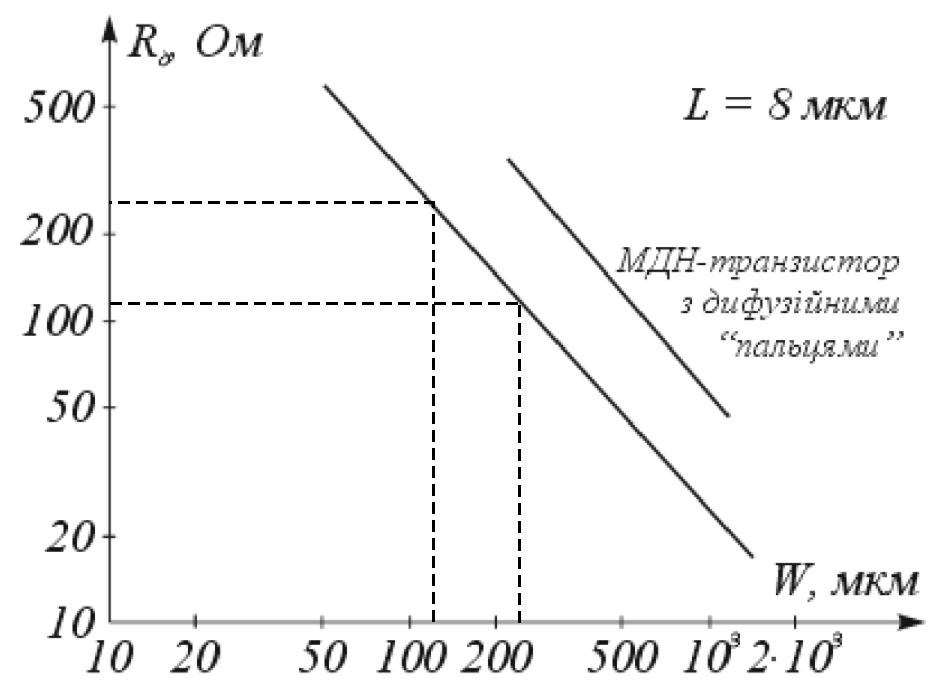
\includegraphics[width=0.8\linewidth]{2-5.png}}
	\caption{Графік для знаходження ширини}
	\label{ris2}
	\end{figure}

	І треба знайти довжину струмообмежуючого опору: $L_{R}=\frac{R_{0} \cdot W_{R}}{\rho_{S}}$, де $\left.W_{R}\right|_{T_{1}, T_{2}, T_{3}}=5 \text{ мкм}$
	- ширина дифузійної шини, $\rho_{S}=100 \text{ Ом}-$ питомий опір дифузійної шини.
	Тоді
	$$
	\begin{array}{c}
	\left.L_{R}\right|_{T_{1}, T_{2}}=\frac{\left.R_{6}\right|_{T_{1}, T_{2}} \cdot W_{R}}{\rho_{S}}=1000 \text{ мкм} \\
	\left.L_{R}\right|_{T_{3}}=\frac{\left.R_{6}\right|_{T_{3}} \cdot W_{R}}{\rho_{S}}=2000 \text{ мкм}
	\end{array}
	$$
	\begin{table}
	\caption{ Таблиця розмірів ПЗ для кожного входу}
	\begin{tabular}{|c|c|c|c|c|c|c|c|}

	\hline & & & & Діод & Діод & Транзистор & Транзистор \\
	& $T_{1}$ & $T_{2}$ & $T_{3}$ & $\left(T_{1}, T_{2}\right)$ & $\left(T_{3}\right)$ & $\left(T_{1}, T_{2}\right)$ & $\left(T_{3}\right)$ \\
	\hline$W$, \text{ мкм} & 110 & 110 & 55 & 238 & 119 & 5 & 5 \\
	\hline L,\text{ мкм} & 5 & 5 & 5 & 5 & 5 & 1000 & 2000 \\
	\hline$W / L$ & 22 & 22 & 10,17 & & & & \\
	\hline

	\end{tabular}

	\end{table}



\newpage
\chapter{ТЕХНОЛОГІЯ ВИГОТОВЛЕННЯ МДН ІС}
	В своїй роботі маю КЕФ-5, що позначає пластини кремнію монокристалічного електронного типу провідності з додаванням фосфором і питомим опором 5 Ом$\cdot$см.\\

	\begin{enumerate}
	\item Проведення підготовки: пластини кремнію шліфують до заданої товщини, потім полірують, піддають травленню і промивають. 



	\item Перша фотолітографія дозволяє розкрити вікна в оксиді для локальної дифузії, в результаті якої формуються області витоку та стоку. Дифузія проводиться в дві
	стадії на глибину 0,5 мкм.\\

	\item Друга фотолітографія проводиться для розкриття вікон під тонкий оксид. Тонкий оксид вирощується на поверхні кремнію в сухому кисні при температурі 1150...1200$^{\circ}$ C.\\

	\item Витравлювання оксиду до кремнію, де будуть знаходитися затвори транзистора.\\

	\item Формування підзатворного діелектрика, розгонка.\\

	\item Третя фотолітографія, тобто формування вікон для майбутніх контвктів.\\

	\item Металізація, нанесення слою алюмінію за допомогою електровакуумного напилення, там де є області алюмінию та кремнію треба ці місця пролегувати $n^+ $ типом, тому що утвориться діод Шотткі.\\

	\item Четверта фотолітогорафія, формування з'єднань на ІМС, формування стоку, витоку, затвору.\\

	\item Хіміко-механічна планеризація, тобто видалення зайвих нерівностей та полірування.\\

	\item Пасивація, утворення тонкого шару алюмінию для захисту від корозії\\

	\item Остання фотолітографія -- відкриття контактних площадок.


\end{enumerate}

\newpage
\chapter{ВИСНОВОК}

\newpage
\chapter{СПИСОК ВИКОРИСТАНОЇ ЛІТЕРАТУРИ }
	\begin{thebibliography}{9}
		\bibitem{lit1} wefvnfjnvdlrfbvndfg2009.
	\end{thebibliography}

\newpage
\chapter{ДОДАТОК А }

\newpage
\chapter{ДОДАТОК B }




\end{document}
